\newpage

\section{Medições em laboratório}

\begin{figure}[h]
    \centering
    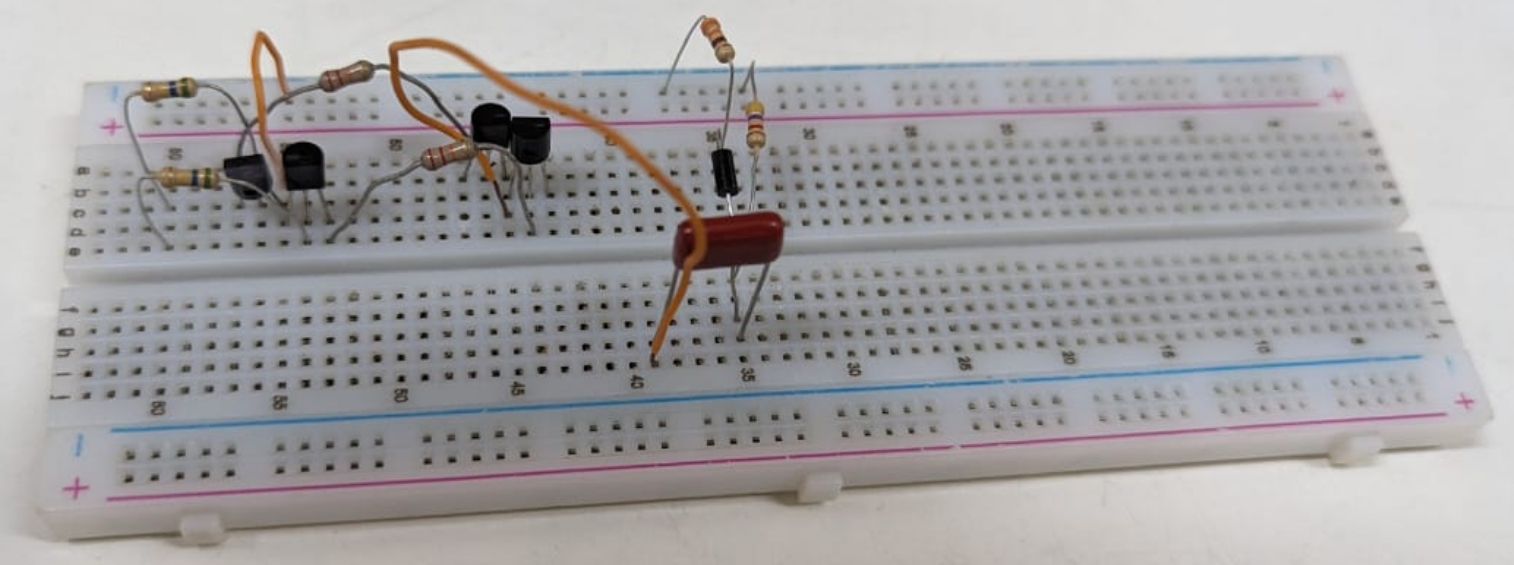
\includegraphics[width=0.7\columnwidth]{images/circuito_montado.png}
    \caption{Imagem do circuito montado em laboratório.}
\end{figure}

Nesta seção, são apresentados os detalhes e resultados das medições realizadas no experimento, com o objetivo de obter dados quantitativos para análise e validação dos resultados teóricos previamente obtidos.

\subsection{Buffer de corrente}

Nesse caso, a corrente necessária para o circuito é maior do que a corrente máxima que o gerador de sinais pode fornecer. Portanto, será necessário utilizar um buffer de corrente. O buffer de corrente é um dispositivo eletrônico que amplifica e fornece a corrente necessária para o circuito de carga, permitindo que o sinal de entrada seja adequadamente amplificado e transmitido sem comprometer a integridade do sinal.

\begin{figure}[h]
    \centering
    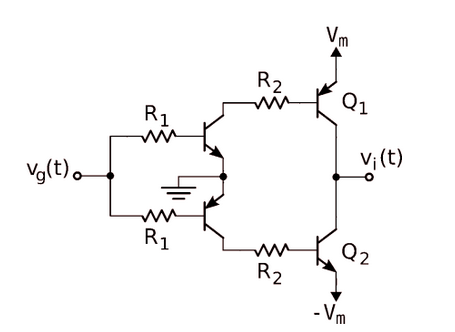
\includegraphics[width=0.7\columnwidth]{images/buffer_corrente.png}
    \caption{Representação esquemática do buffer de corrente utilizado.}
\end{figure}

\subsection{Componentes}

\begin{figure}[h]
    \centering
    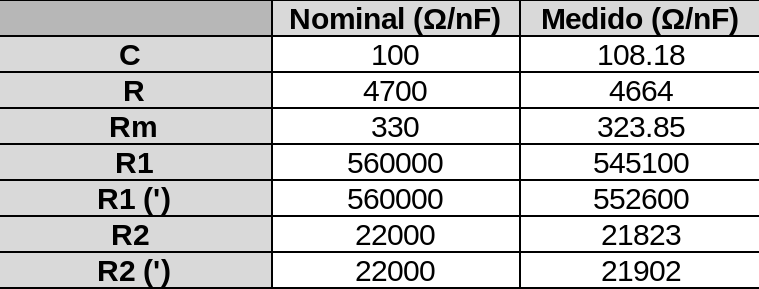
\includegraphics[width=0.7\columnwidth]{images/componentes_reais.png}
    \caption{Representação esquemática do buffer de corrente utilizado.}
\end{figure}

\subsection{Exemplo 1}

Neste exemplo montamos sem o resistor $R$, para simular a situacao de resistencia infinita.

\subsubsection{Gráfico de Vo(t)}

\begin{figure}[H]
    \label{fig:ex1}
    \centering
    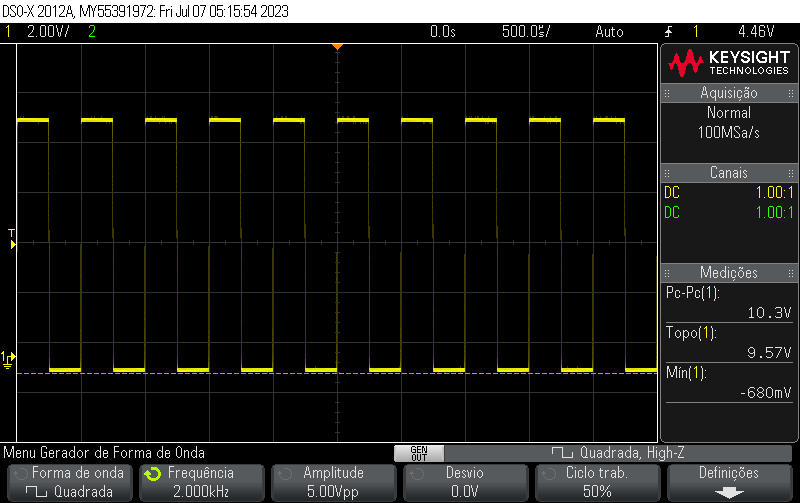
\includegraphics[width=0.7\columnwidth]{images/exemplo1.png}
    \caption{Medição de Vo(t) vista no osciloscópio para $0 < t < 5 T_s$.}
\end{figure}

\subsubsection{Mínimos e máximos.}

\begin{figure}[H]
    \label{fig:minmax_ex1}
    \centering
    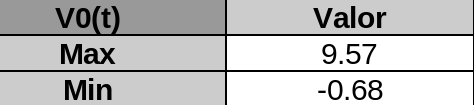
\includegraphics[width=0.5\columnwidth]{images/minmax_ex1.png}
    \caption{Tabela de mínimos e máximos do exemplo 1.}
\end{figure}

\newpage

\subsection{Exemplo 2}

Neste exemplo montamos com um resistor  de $4.7K \Omega$.

\subsubsection{Gráfico de Vo(t)}

\begin{figure}[h]
    \label{fig:ex2}
    \centering
    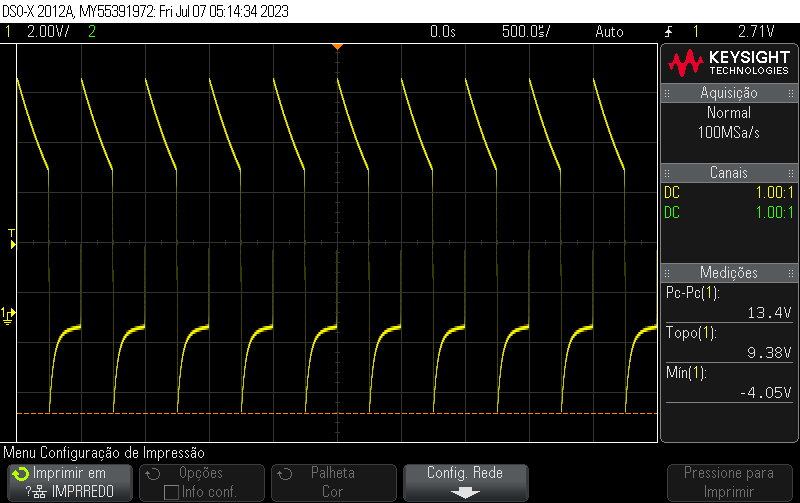
\includegraphics[width=0.7\columnwidth]{images/exemplo2.png}
    \caption{Medição de Vo(t) vista no osciloscópio para $0 < t < 5 T_s$.}
\end{figure}

\subsubsection{Mínimos e máximos.}

\begin{figure}[h]
    \label{fig:minmax_ex2}
    \centering
    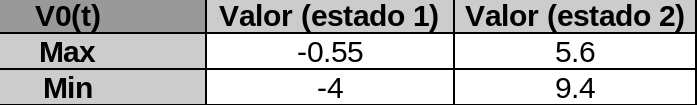
\includegraphics[width=0.5\columnwidth]{images/minmax_ex2.png}
    \caption{Tabela de mínimos e máximos do exemplo 2.}
\end{figure}


